\section{Motivation}

Sind Soldaten auf einem Marshc müssen sie vor bestimmten Brücken ihren Gleichschritt unterbrechen.
Warum das so ist soll dieser Versuch verdeutlichen. Entspricht nämlich die Schrittfrequenz genau der Eigenfrequenz der Brrückenkonstruktion,
kann es zur Resonanzkatastrophe kommen, sodass die Brücke enstürzen kann. Durrch die Anzahl der Leute wird eine ausrechende Amplitude erzeut, welche sich durch die 
Resonanz so weit aufschaukeln kann, dass das Bauwerk der Belastung nicht mehr standhalten kann.

\section{Messverfahren}

Für diesen Versuch wird ein Drehpendel mit einer Skala und angeschlossenem Schrittmotor verwendet.
Die Frequenz des Schrittmotors kann über einen Funktionengenerator eingestellt werden.
Das Pendel wird durch Spulen mithilfe von Wirbeströmen gebremst. Die Dämpfung kann über eine Spannungsquelle angepasst werden.

\section{Grundlagen aus der Physik}
\subsection{Gedämpfter harmonische Oszillator}

Für die Amplitude $A$ gilt in einemgedämpften Pendel mit $A_0$ als Ausgangsamplitude und $\delta$ als Dämpfungskonstante:
\begin{equation}
    A(t) = A_0 e^{-\delta t} \sin(\omega_f t)
\end{equation}
Hier bezeichnet $\omega_f$ die Winkelfrequenz des gedämpften Oszillators.
\subsection{Bestimmung der Dämpfung durch die Halbwertszeit der Amplitude}

Die Dämpfungskonstante $\delta$ kann bestimmt werden, wenn die Zeit für die halbierung der Amplitude $t_{1/2}$ bekannt ist.
In diesem Fall kann sie Brechnet werden durch die Periodendauer $T$, welche unabhängig von der Amplitude ist, und der Halbwertsanzahl der Amplitude $n_{1/2}$.
Also die Anzahl der Schwingungen für die Halbierung der Amplitude.
\begin{align}
    \delta &= \frac{\ln 2}{t_{1/2}} \\
    t_{1/2} &= T  \cdot n_{1/2} \\
    \Rightarrow \delta &= \frac{\ln 2}{T  \cdot n_{1/2}}
    \label{eq:delta}
\end{align}

\subsection{Bestimmung der Dämpfung durch die Halbwertsbreite}

Für die Eigenfrequenz des Pendels gilt mit $T$ als Periodendauer:
\begin{equation}
    \omega_0 = \frac{2\pi}{T} = 2 \pi f
    \label{eq:eigen}
\end{equation}
Die Halbwertsbreite ist der Abstand der Frequenzen $\omega_1$, $\omega_2$ bei denen die halbe Maximalamplitude abgelesen werden kann.
Bei nicht zu starker Dämpfung gilt folgende Gleichung:
\begin{equation}
    H = (\omega_2-\omega_1) = 2\delta
    \label{eq:halb}
\end{equation}

\subsection{Bestimmung der Dämpfung durch die Resonanzüberhöhung}
Für $\omega'$ also die Frequenz bei maximaler Amplitude bzw die Resonanzfrequent kann bestimmt werden durch:
\begin{equation}
    \omega' = \sqrt{\omega_0^2 - 2\delta^2}
\end{equation}

Für die Amplitude des Drehpendels gilt in Abhänigkeit der Anregungsfrequenz:
\begin{equation}
    b(\omega) = \frac{A\omega_0^2}{\sqrt{(\omega_0^2-\omega^2)^2 - (2\delta\omega)^2}}
\end{equation}

Lässt man nun $\omega$ gegen 0 laufen so erhält man die messbare Amplitude zu Beginn der Messung, für welche gilt:

\begin{equation}
    b(\omega \rightarrow 0) = A \omega_0
\end{equation}

Die Resonanzüberhöhung ist nach Umstellung nach $\delta$ definiert durch:

\begin{equation}
    \delta = \frac{\omega_0 \cdot b(\omega \rightarrow 0)}{2 \cdot b(\omega')}
    \label{eq:deltafertig}
\end{equation}

\section{Aufbau}
\begin{figure}[h!]
    \centering
    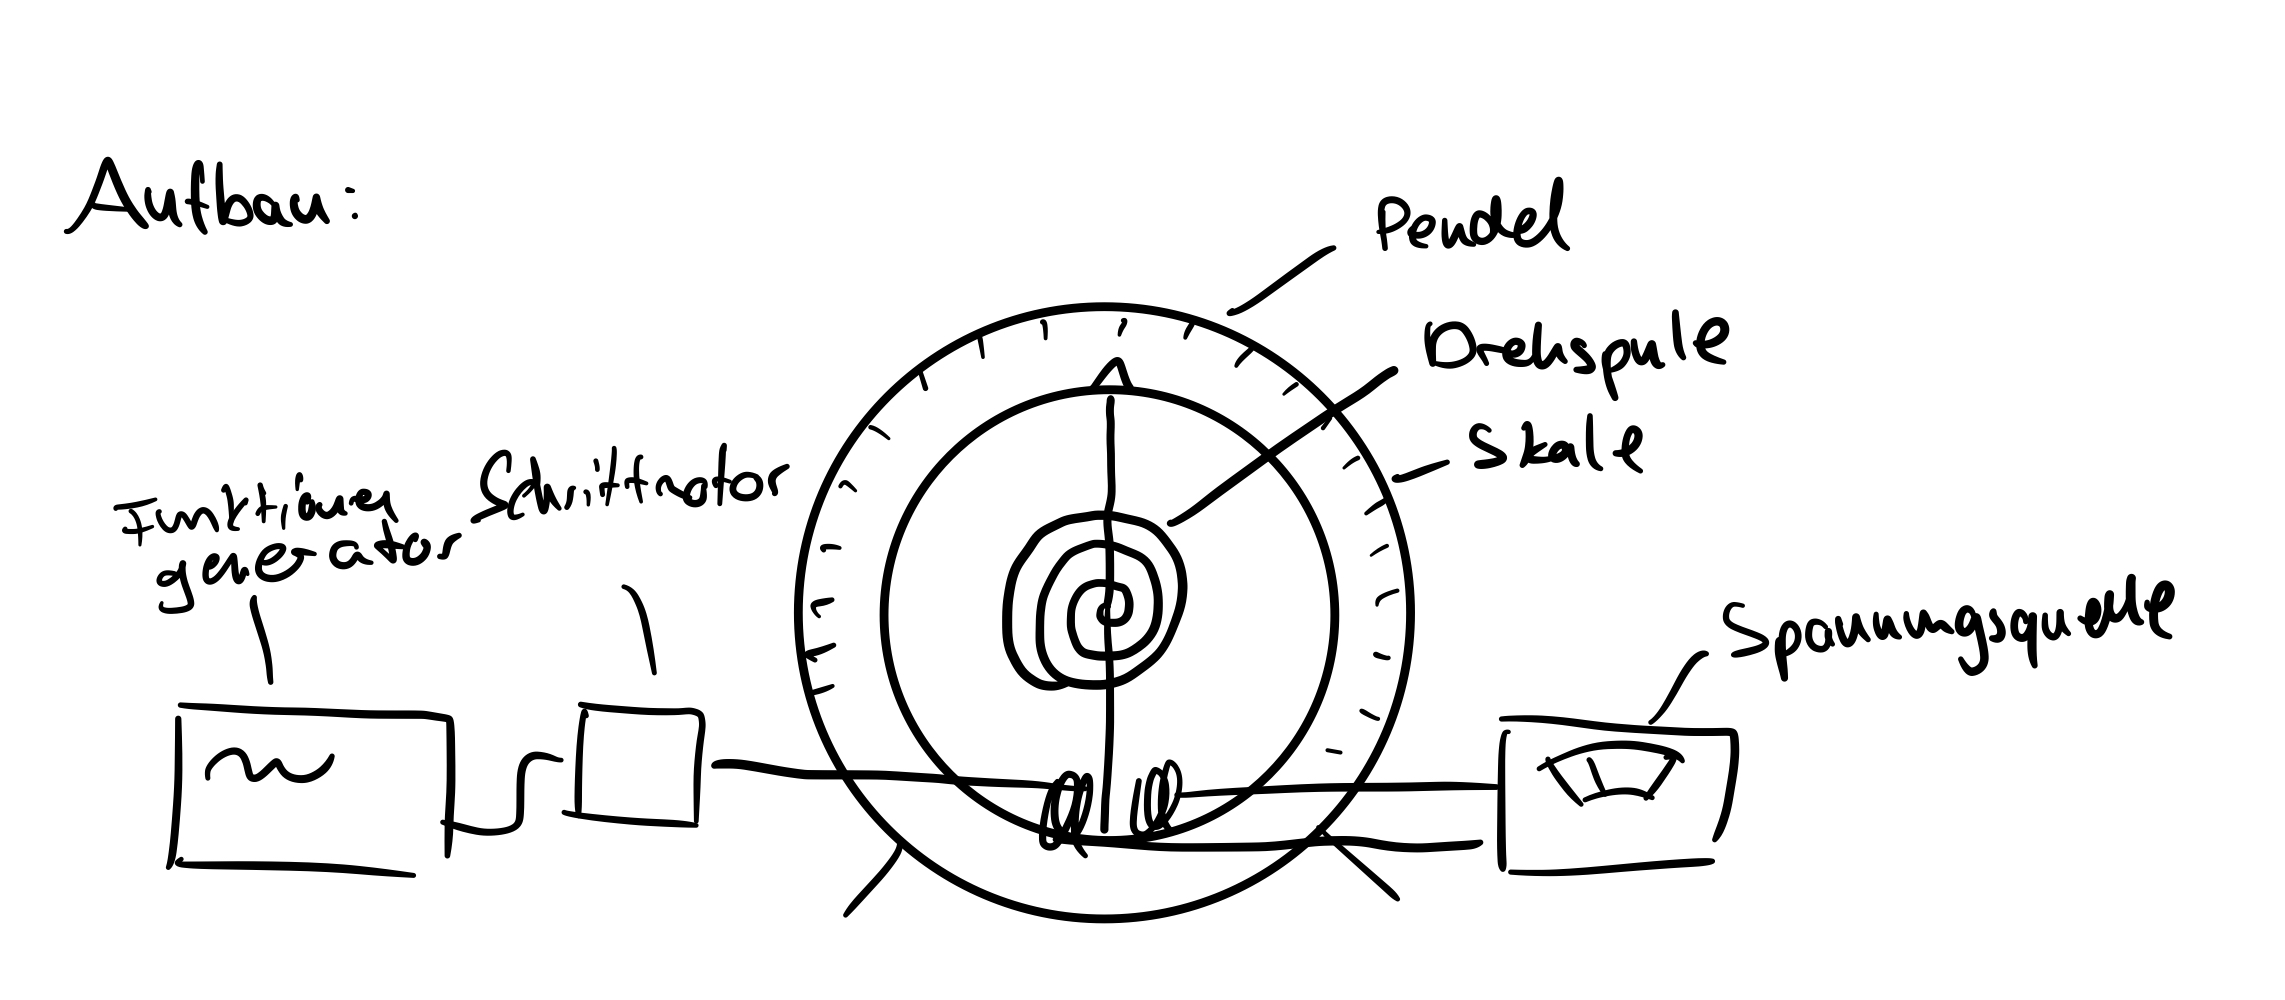
\includegraphics[width = .5 \textwidth]{IMG_178CE5573475-1.jpeg}
    \caption{Aufbau}
\end{figure}